\documentclass[a4paper]{article}

%% Language and font encodings
\usepackage[english]{babel}
\usepackage[utf8x]{inputenc}
\usepackage[T1]{fontenc}
%\usepackage{natbib}
\usepackage{algorithm}
\usepackage{algorithmic}
\setlength{\parindent}{0pt}

%% Sets page size and margins
\usepackage[a4paper,margin=2cm]{geometry}

%% Useful packages
\usepackage{para list}
\usepackage{booktabs}
\usepackage{multirow}
\usepackage{clrscode}
\usepackage{listings}
\usepackage{multicol}
\usepackage{textcomp}
\usepackage{amsmath}
\usepackage{graphicx}
\usepackage[colorinlistoftodos]{todonotes}
\usepackage[colorlinks=true, allcolors=blue]{hyperref}
\usepackage{booktabs}
\newcommand{\tabincell}[2]{\begin{tabular}{@{}#1@{}}#2\end{tabular}}

% This will make it easier for markers
% to refer to specific lines of your report.
\usepackage{lineno}
\linenumbers 

\title{Beam Search with Different Prune and Normalisation methods \\
-- Apply beam search to Inutitut NMT model}
% Your report should be anonymous: it should not
% contain your name(s) or student id(s).
\date{}

\begin{document}
\maketitle

\begin{abstract}

As describe in the possible extensions for homework 2, it introduces some unsolved problems and introduces the possible way to improve the translation quality by some ways, such as the beam search, the more peaky a distribution, the more certain the model is about the choice of next output word.So we would like to do deeper research in the beam search. For each step in the decoder, we would like to explore the probability distribution over the English vocabulary. Meanwhile, we would like to extract the top k number of most probable translations and see whether the correct word is included in these translations. On the base of training model of RNN, with LSTM, attention mechanism by Sequence-to-Sequence (seq2seq) modeling with greedy search, we would like to implement the basic beam search at the first stage. Then we would like to try the pruning method(relative prune and absolute prune) to see whether it could improve the translation performance. Moreover, some normalisation methods(length penalty) will be applied into the model. Finally, we find combining beam search with greedy search could help to improve the beam search performance.


\end{abstract}

\section{Introduction}
\subsection{Dataset}
In this assignment, we would like to translate Inuktitut, which is the polysynthetic language. The data comes from the Legislative Assembly of Nunavut, which publishes its Hansard in both English and Inuktitut[2].

With the analysis of the source data, we find that several interesting things:
\begin{enumerate}
\item The number of tokens in English is 459895 and that of Inuktitut is 222757. This will cause the problem that the model might find many candidate hypothesises for one Inuktitut word and finally result in bad translations.
\item The word type of English sentences is 9996 while that of Inuktitut is 72734 which is much larger than English. This phenomenon will cause the model hard to find the alignments.
\item As for the unknown tokens, English sentences have 3552 unknown tokens and Inutitut sentences have 59254 unknown tokens. This unbalance will cause difficulties in predicting process. For example, the more unknown tokens in a source sentence, the more inaccurate the translation is.
\end{enumerate}

\subsection{Baseline}
The provided baseline is a RNN model with LSTM units. The model contains 3 layers of encoder and 3 layers of decoder and each layer contains 400 units. The soft attention mechanism is also applied to the model to overcome the poor performance on long sentence. The model is trained for 50 epochs with Adam optimiser and the 19th model is choose for it has best BLEU score. The translation results are not very well for the BLEU of the model is only 7.98. In this assignment, we will continue using the BLUE score as the main metric to evaluate the performance of the model. The detailed statistics of the baseline model is shown in Table 3(refer to Appendix Table 3).

\subsection{Motivation}
When we analyze the translation result of the baseline model, we find that the correct translation result exists in the candidate hypothesises. We plot the top 5 hypothesises of each source word. The red words in the word hypothesises are the original hypothesis, the arrows in the plot shows the correct translation that exists in the hypothesis space.  
\begin{center}
\begin{tabular}{r l}
Src & uuviq alakkannuaq \\
Ref & mr ovide alakannuark \\
Original Hyp & ovide dorset alakannuark \_EOS
\end{tabular}
\end{center}

\begin{figure}[h]
\begin{center}
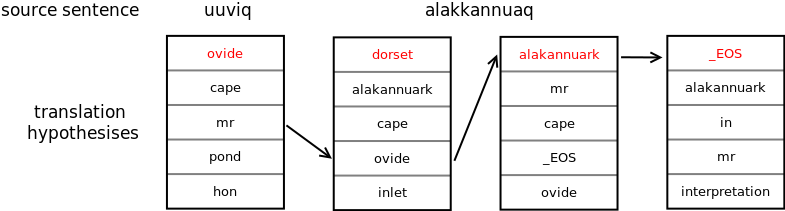
\includegraphics[width=5in]{translation_hyp}
\caption{Translation result and candidate translation hypothesises}
\end{center}
\end{figure}
We could find that the correct hypothesis is the third candidate in the hypothesises and the correct hypothesis for the second word is the forth hypothesis. Therefore, we think that the problem that exists in the baseline model is not the model structure but the process to generate the hypothesis. To solve this problem, we motivate this assignment by searching the correct translation among the translation candidates. Through our reading of related papers, beam search is one of the effective methods to handle such situation.

In 2014, the researchers Sutskever et al.[1] introduce the Sequence-to-Sequence learning with deep neural networks, which has rapidly become a very useful and surprisingly general-purpose tool for natural language processing. M. Freitag and Y. Al-Onaizan[2] introduce the beam search strategies for neural machine translation. In this paper, based on the original beam search decoder in Neural Machine Translation, it introduces several pruning techniques which prune candidates whose scores are far away from the best one and it finally speed up the decoder by up to 43\%. With the basis of this paper, we implement beam search and test different beam search strategies to see if this technology could help to improve the baseline model.



\section{Measures and Methods}

\subsection{Basic Beam Search}
The Algorithm 1(refer to Appendix Algorithm 1) is the pseudocode of the original beam search. The input of function is the encoder, decoder and input sentence $x$, we try to find the translation based on the log probability $y =argmax_y p(y|x)$. A group of stacks are used to store hypotheses during the searching. \textbf{beam\_size} is used to control the search space by extending the top several hypotheses in the current stack.\textbf{complete\_hypothesis} is used to store the hypothesis which has already reach the end of the sentence "EOS".

% \begin{table}
% \centering
% \begin{tabular}{lr}\hline\hline
% Item & Quantity \\\hline
% Widgets & 42 \\
% Gadgets & 13
% \end{tabular}
% \caption{\label{tab:widgets}An example table.}
% \end{table}

\subsection{Pruning}
The original beam search method will dramatically slow down the predict process (it often takes several hours to compute the BLEU score for the 5000 sentences of dev dataset). Therefore, pruning tricks are needed to improve the speed of the prediction process. Markus(2017) introduces several pruning methods in his paper. The pruning thresholds could be defined as relative threshold and absolute threshold. The relative threshold allows the hypothesis to be worse than the best one in the stack. If the probability of a hypothesis is $\alpha$ times worse than the best hypothesis, it is pruned out. The absolute threshold prunes the hypothesises that is worse than a fixed threshold. We will use these two pruning schemes in this assignment.

\textbf{Relative Threshold Pruning.} The relative threshold abandons candidates which are far worse than the best active candidate. Suppose there is a pruning threshold $rt$ and candidate list $L$, and a candidate $a\in L$ is abandoned if:
\begin{align*}
score(a) \leq rt*argmax_{l \in L}\{score(l)\} \qquad where \qquad  l \in L
\end{align*}
Refer to Markus's(2017) work, we set the $rt$ to 0.3.

\textbf{Absolute Threshold Pruning.} In absolute threshold pruning, we abandon candidates when they are worse by a specific threshold than the best active candidate. Suppose there is a pruning threshold $at$ and candidate list $L$, and a candidate $a\in L$ is abandoned if:
\begin{align*}
score(a) \leq argmax_{l \in L}\{score(l)\}-at \qquad where \qquad  l \in L
\end{align*}
Also, according to Markus's(2017) work, we set $at$ to 0.25.

%\textbf{Relative Local Threshold Pruning}. In relative local threshold pruning, we abandon candidates only consider the score $score_{s}$of the last generated word instead of the total score. Suppose there is a pruning threshold $rlt$ and candidate list $L$, and a candidate $a\in L$ is abandoned if:
%\begin{align*}
%score_{s}(a) \leq rlt*argmax_{l \in L}\{score_{s}(l)\} \qquad where \qquad  l \in L
%\end{align*}

\subsection{Normalization}
%\subsubsection{Length Normalization}
In 2015, the researchers, X. Hu et al [5] in Baidu Inc introduce a way to add the length penalty to beam search for NMT. In this paper, the researchers found that it is unfair directly to compare the translation probabilities of hypotheses by the reason that the longer translation often tend to get lower probability.  We would like to implement the length penalty in this project and we would like to refer the formula in this paper[5].
\begin{align*}
\widetilde p(y|x)=p(y|x)^{\frac{1}{1+\alpha * (i-1)}}
\end{align*}
where $\alpha$ is use to alleviate the influence of translation length and i is the length of hypothesis. The lower the $\alpha$ is, the less hypothesis will be pruned. According to Hu's work, the value of $\alpha$ is usually 1 and it could give the best result.

\subsection{Implementation}
We implement beam search by changing the $decoder\_predict$ function. The beam search is only used for searching the best translation. Follow the pseudocode and optimization methods, we implement beam search and set $BEAM\_SIZE$ and $NORM\_A$ as the hyper-parameters to control the beam search process. In our experiments, we will test the performance of different beam search strategies.

\section{Results and Analysis}

\subsection{Experiment design}
With the implementation of beam search, we design a group of experiments to test the performance of beam search. The design of the experiments is shown in Table 4 (refer to Appendix Table 4). We want to estimate the effects of different prune strategies and normalisation methods.

Through the result of the experiments, we could investigate that with the increase of beam size, the performance of beam search gets better and it will get stable after some point.By comparing different prune strategies, we find that absolute threshold cost less time than relative threshold and they both achieve similar result on BLEU. However, length normalisation doesn't provide any improvement of beam search.

\subsection{Analysis of Long Sentence}
With the observation of our first attempt of beam search, we find that the beam search strategy always stacks on long sentences because the long length of source sentence will make it hard to generate translations and even worse, long source sentences will lead to an empty $complete\_hypothesis$. Even though it finishes the searching process, the translation results are always bad. For example, have a look at the below translation.
\begin{center}
\begin{tabular}{r l}
Src &  \tabincell{l}{pinasuarnirijatigut assuuruutigijavut ammalu ujjiunngittumit aturnirijavut \\ katimajiuqatittinnut asinginnullu gavamaujunit ilippaallirutaunaasuqput} \\
Ref &  \tabincell{l}{our distinct challenges and unique experiences are something that our colleagues \\ and other governments are eager to learn about} \\
Original Hyp & \_UNK \_UNK \_UNK training and \_UNK \_UNK \_UNK \_UNK \_UNK \_UNK \_EOS \\
Beam Search Hyp & \_UNK \_EOS \\
\end{tabular}
\end{center}
From the above translation, we could investigate that the original model result is very bad because the hypothesis is far away from the reference. And the beam search result is nearly an empty result for the reason that the candidate hypothesises is discarded. So, instead of generating empty hypothesis, we combine the beam search with greedy search for the purpose that if the model generate empty hypothesis, the greedy search strategy will be used to give result. Since the prune threshold will only influence the time cost of decode process, we will only use absolute threshold(0.25) in further experiments. Our new experiments and results about new search strategy are shown in below table(Table 1).

\begin{table}[H]
\centering
\caption{The Experiments Design of Combined Search Strategy}
\label{my-label}
\begin{tabular}{c c c c c c}
\toprule
Beam size & Absolute threshold & $NORM\_A(\alpha)$ & Time cost(run on DICE) & BLEU  \\ 
2 & 0.25 & 0 & 9m49s & 7.15 \\ 
3 & 0.25 & 0 & 10m25s & 7.16 \\ 
4 & 0.25 & 0 & 10m16s & 7.16 \\ 
2 & 0.25 & 1 & 4h48m & 6.54 \\
3 & 0.25 & 1 & 5h13m & 6.58 \\
\bottomrule
\end{tabular}
\end{table}

By analysing the results, we investigate that the combined strategy could effectively improve the performance of the model. And the normalisation parameter will also effect the performance although the BLEU score gets down. We think the reason to this is that the normalisation of probability will force the translation results get longer which in this case leads to bad translation results. On the other hand, the time consuming gets longer with normalisation method. In conclusion, simple length normalisation of probability seems not suitable for this model.

Finally, we compare our best performing model across all experiments and choose the best parameters to have the final translation output. Table 2 shows our final model, consisting of all the best optimized values. 
\begin{table}[H]
\centering
\caption{Hyper-parameter settings for our final
model, consisting of all of the individually
optimized values.}
\begin{tabular}{@{}cccccccc@{}}
\toprule
Rnn cell & Encoder & Decoder & Attention      & Beam size &  Absolute threshold & Normalisation & BLEU \\ \midrule
LSTM     & 3 layer & 3 layer & Soft Attention &     3     &        0.25         &      without normalisation & 7.16 \\
\bottomrule
\end{tabular}
\end{table}

However, our results doesn't like what we find from the reference papers -- beam search would provide significant improvement of the translation results. Applying beam search to our baseline model could reach the BLEU of 7.16. We think one possible reason to this might relate to the model itself. The model doesn't give higher probability to the correct translation result when the beam search scans through it. As what we observed from the source data, the unbalance of training data make the model hard to fit the data. Hence, if we want to improve the translation performance by beam search, we need to create a better model. 

\section{Conclusion and Future Work}
In this assignment, we implement beam search which based on the provided baseline model and test different prune strategies and length normalisation method. Although the beam search method doesn't improve the translation performance of Inutitut baseline model, we still have some interesting findings. Hence, we conclude our practical findings as follow:
\begin{enumerate}
\item In terms of beam size, we find that with the increase of beam size, the translation results get better. After the beam size is bigger than a value, the performance gets stable.
\item Prune strategies(relative prune and absolute prune) could effectively speed up the beam search process, which makes beam search executable.
\item Length normalisation method might make the translation performance worse because it forces the translation of short sentences get longer.
\item Combined beam search with greedy search could provide significant improvement of the translation result, which is our best result in this assignment. 
\item Generally, beam search may not improve the performance of the model even we could find the correct candidate hypothesises because the model doesn't fit the language well and gives lower probability to the correct translation result.
\end{enumerate}

For future work, I think we could improve the model from below aspects:
\begin{enumerate}
\item \textbf{Different normalisation tricks.} Since length normalisation doesn't provide good results and the problem of translating long sentence still exists, different normalisation methods could be a good aspects to test the beam search performance.
\item \textbf{Pre-process source data.} Due to the characteristics of Inutitut, the number of token type of Inutitut is much larger than English, which will make the model hard to fit the data. To do this, splitting the Inutitut word into small sub word could effectively reduce the number of token type and make it easier to find the alignments. Therefore, pre-process the source data by splitting the word worth a trying in future work.
\item \textbf{Character level model.} Similar to the pre-process, character level model could also solve the problem caused by unbalanced source data since the features that entries the encoder-decoder are generated from characters, which will significantly reduce the number of word tokens.  
\end{enumerate}


% \subsection{How to write Mathematics}  

% \LaTeX{} is great at typesetting mathematics. Let $X_1, X_2, \ldots, X_n$ be a sequence of independent and identically distributed random variables with $\text{E}[X_i] = \mu$ and $\text{Var}[X_i] = \sigma^2 < \infty$, and let
% \[S_n = \frac{X_1 + X_2 + \cdots + X_n}{n}
%       = \frac{1}{n}\sum_{i}^{n} X_i\]
% denote their mean. Then as $n$ approaches infinity, the random variables $\sqrt{n}(S_n - \mu)$ converge in distribution to a normal $\mathcal{N}(0, \sigma^2)$.


% \subsection{How to create Sections and Subsections}

% Use section and subsections to organize your document. The sections and subsections create an outline of your report, and a reader should be able to infer the structure of your report just by skimming them.

\newpage
\begin{thebibliography}{9}
\bibitem{Sutskever2014}
  I. Sutskever, O. Vinyals, and Q. Le. 
  Sequence to sequence learning with neural networks. 
  In Advances in Neural Informa- tion Processing Systems (NIPS), pages 3104–3112, 2014.
\bibitem{Markus2017}
  Markus Freitag and Yaser Al-Onaizan. 
  Beam Search Strategies for Neural Machine Translation. arXiv:1702.01806, 2017.
\bibitem{datasource}
  http://www.inuktitutcomputing.ca/index.php
\bibitem{cw3}
  http://www.inf.ed.ac.uk/teaching/courses/mt/hw2.html
\bibitem{Hu2015}
  X. Hu, W. Li, X. Lan,H. Wu,H. Wang. 
  Improved Beam Search with Constrained Softmax for NMT. 
  Proceedings of MT Summit XV, vol.1: MT Researchers' Track, 2015.
\end{thebibliography}


% [1] W. Ling, I. Trancoso, C. Dyer, A. W Black. Character-based Neural Machine Translation. arXiv:1511.04586v1, 2015.

% [2]J. Lee, K. Cho, and T. Hofmann. Fully character-level neural machine translation without explicit segmentation. arXiv preprint arXiv:1610.03017, 2016.
%[2]Markus Freitag and Yaser Al-Onaizan. Beam Search Strategies for Neural Machine Translation. arXiv:1702.01806, 2017.
%
%[3]http://www.inuktitutcomputing.ca/index.php 
%
%[4]http://www.inf.ed.ac.uk/teaching/courses/mt/hw2.html
%
%[5]X. Hu, W. Li, X. Lan,H. Wu,H. Wang. Improved Beam Search with Constrained Softmax for NMT. Proceedings of MT Summit XV, vol.1: MT Researchers' Track, 2015.
\newpage
\section*{Appendix}

\begin{algorithm}
  \caption{Basic Beam Search}
  \begin{algorithmic}[1]
  \REQUIRE input $enc,dec,x,y$
  %\STATE \textbf{function} original\_beam\_search(enc,dec,x,y)
  \STATE define $beam[[]]$
  \STATE define complete\_hypothesis
  \STATE create initial hypo and put it into beam[0]
  \STATE pred\_count ← 0
  \STATE N ← beam size
  \WHILE{$beam[pred\_count] \neq ∅ $}
  \FORALL{$h \in beam[pre\_count] $}   \STATE extend N hypos from h
  \STATE put new hypos into beam[pre\_count + 1]
  \IF{the hypos reaches the end $\_EOS$} 
  \STATE put the complete hypo to complete\_hypothesis and remove it from beam
  \ENDIF
  \ENDFOR
  \ENDWHILE 
  \STATE y ← trace back from best h ∈  complete\_hypothesis
  %\STATE \textbf{end function}
  \end{algorithmic}
\end{algorithm}

\begin{table}[H]
\centering
\caption{The Statistics of Baseline Model}
\label{my-label}
\begin{tabular}{@{}lllll@{}}
\toprule
Models & Architecture & Attention      & Units & BLUE \\ \midrule
RNN+LSTM    & 3-3layer     & Soft Attention & 400   & 7.98          \\ \bottomrule
\end{tabular}
\end{table}

\begin{table}[H]
\centering
\caption{The Experiments Design of Beam Search}
\label{my-label}
\begin{tabular}{c c c c c c}
\toprule
Beam size & Relative threshold & Absolute threshold & $NORM\_A(\alpha)$ & Time cost (run on DICE)& BLEU  \\ 
\midrule
1 & $\times$ & $\times$ & 0 & 6m17s & 7.99 \\
\midrule
2 & $\times$ & $\times$ & 0 & 3h20m & 6.19 \\
2 & $\times$ & 0.25 & 0 & 8m24s & 6.19 \\
3 & $\times$ & 0.25 & 0 & 8m58s & 6.68 \\
4 & $\times$ & 0.25 & 0 & 9m05s & 6.68 \\
\midrule
2 & 0.3 & $\times$ & 0 & 8m37s & 6.19 \\
3 & 0.3 & $\times$ & 0 & 9m10s & 6.68 \\
4 & 0.3 & $\times$ & 0 & 9m52s & 6.68 \\
\midrule
3 & $\times$ & 0.25 & 1 & 4h42m & 6.04 \\
3 & 0.3 & $\times$ & 1 & 4h51m & 6.04 \\
\bottomrule
\end{tabular}
\end{table}


\end{document}